\documentclass[a4paper]{article}
\usepackage[T1]{fontenc} 
\usepackage[utf8]{inputenc}
\usepackage{graphicx}
\usepackage{float}
\usepackage[czech]{babel}
\usepackage[export]{adjustbox}

\setlength{\hoffset}{-2cm} 
\setlength{\voffset}{-2cm}
\setlength{\textheight}{24.0cm} 
\setlength{\textwidth}{17cm}

\begin{document}

\flushleft
\large
\textbf{Jméno:} Karel Norek

\textbf{Login:} xnorek01

\textbf{Přístupové kódy:} 1. Kód = 879872350, 2. Kód = 8798752533

\vspace{0.5cm}

\Large \textbf{Vstupní/výstupní signály}

\vspace{0.2cm}
\large
Legenda vstupních signálů:
\begin{itemize}
    \item K : KEY
    \item CO: CNT\_OF
\end{itemize}

Identifikace výstupních signálů
\begin{itemize}
    \item Mealyho výstupy: FSM\_LCD\_WR, FSM\_LCD\_CLR 
    \item Moorovy výstupy: FSM\_CNT\_CE, FMS\_MX\_MEM, FMS\_MX\_LCD
\end{itemize}

\vspace{0.2cm}
\Large \textbf{Graf přechodů:}

\begin{figure}[H]
    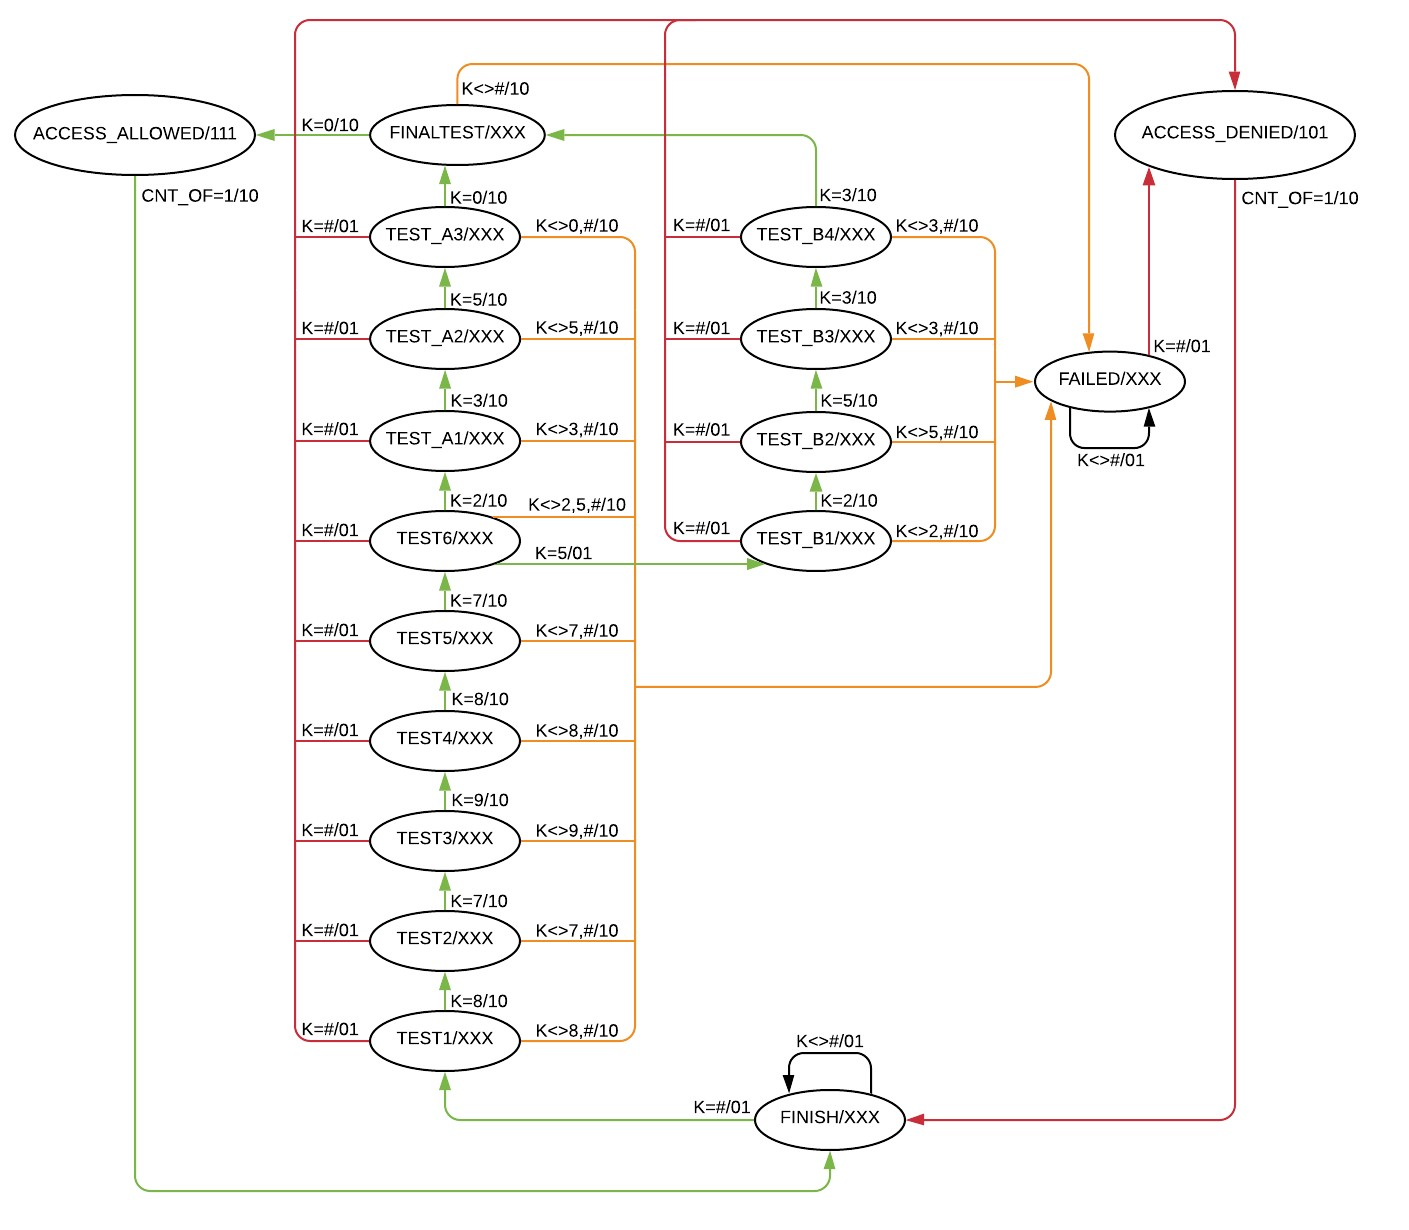
\includegraphics[scale=0.75, keepaspectratio]{graf.jpg}
    \label{fig:Graf}
\end{figure}

\end{document}
